\documentclass{sciposter}


\usepackage{epsfig}
\usepackage{amsmath}
\usepackage{amssymb}
\usepackage{multicol}
\usepackage{xcolor}

%\usepackage{fancybullets}

\newtheorem{Def}{Definition}

%\definecolor{BoxCol}{rgb}{0.9,0.9,0.9}
% uncomment for grey background to \section boxes
% for use with default option boxedsections

%\definecolor{BoxCol}{rgb}{0.9,0.9,1}
% uncomment for light blue background to \section boxes
% for use with default option boxedsections

%\definecolor{SectionCol}{rgb}{0,0,0.5}
% uncomment for dark blue \section text

\newcommand{\ud}[1]{{#1^{\dagger}}}
   \newcommand{\bra}[1]{\left\langle #1\right|}
   \newcommand{\ket}[1]{\left| #1\right\rangle}
   \newcommand\Tr{\mathrm{Tr}}
   \newcommand{\braket}[2]{\langle #1 \mid #2 \rangle}
   \newcommand{\avg}[1]{\left< #1 \right>}





\title{Reminder}

% Note: only give author names, not institute
\author{Lei Ma}

% insert correct institute name
\institute{Department of Physics and Astronomy,\\
           University of New Mexico\\}

\email{leima@unm.edu}  % shows author email address below institute

%\date is unused by the current \maketitle


% The following commands can be used to alter the default logo settings
%\leftlogo[0.9]{logoWenI}{  % defines logo to left of title (with scale factor)
%\rightlogo[0.52]{RuGlogo}  % same but on right

% NOTE: This will require presence of files logoWenI.eps and RuGlogo.eps,
% or other supported format in the current directory
%%%%%%%%%%%%%%%%%%%%%%%%%%%%%%%%%%%%%%%%%%%%%%%%%%%%%%%%%%%%%%%%%%%%%%%%%%%%%%%%
%%% Begin of Document



\begin{document}
%define conference poster is presented at (appears as footer)

\conference{{\bf 2015-11-10}}

%\LEFTSIDEfootlogo
% Uncomment to put footer logo on left side, and
% conference name on right side of footer

% Some examples of caption control (remove % to check result)

%\renewcommand{\algorithmname}{Algoritme} % for Dutch

%\renewcommand{\mastercapstartstyle}[1]{\textit{\textbf{#1}}}
%\renewcommand{\algcapstartstyle}[1]{\textsc{\textbf{#1}}}
%\renewcommand{\algcapbodystyle}{\bfseries}
%\renewcommand{\thealgorithm}{\Roman{algorithm}}

%\maketitle

%%% Begin of Multicols-Enviroment
\begin{multicols}{3}

%%% General

\section{General}


\subsection{Units and Conventions}

\begin{enumerate}
\item Energy and temperature: \begin{equation}
\frac{1}{40}\mathrm{eV} = 300\mathrm{K} k_B .
\end{equation}
\item Natural units: energy is related to length by
\begin{equation}
1\mathrm{fm}\times 197\mathrm{MeV}=\hbar c = 1.
\end{equation}

As a reference, $1 \mathrm{GeV} =& 5.08 \times 10^{15} \mathrm {m^{-1}}$.
\item Fermi constant is $G_{\mathrm F}/(\hbar c)^3 = 1.166\times 10^{-5}\mathrm{GeV^{-2}}$.
\item Some ancient astrophysicists like the unit erg, which is $10^{-7}\mathrm{J}$.
\item For light, energy 1eV corresponds to wavelength $1.24\mathrm{\mu m}$.
\item Pauli matrices are
\begin{equation}
    \sigma_1 = \begin{pmatrix} 0 & 1 \\ 1 & 0 \end{pmatrix}, \sigma_2 = \begin{pmatrix} 0 & -i \\ i & 0 \end{pmatrix},\sigma_3 = \begin{pmatrix} 1 & 0 \\ 0 & -1 \end{pmatrix}.
\end{equation}
\item Transformations of Pauli matrices

\begin{align}
\mathbf{U}^\dagger \sigma_3 \mathbf{U} &= \cos 2\theta \sigma_3 + \sin 2\theta \sigma_1 \\
\mathbf{U}^\dagger \sigma_1 \mathbf{U} &= -\sin 2\theta \sigma_3 + \cos 2\theta \sigma_1 \\
\mathbf{U}^\dagger \sigma_2 \mathbf{U} &= \sigma_2.
\end{align}

\end{enumerate}




\subsection{Check Results}

\begin{enumerate}
    \item Are the dimensions correct?
    \item Do the limits of the result make sense?
    \item Does the result make sense when the complexity of the system is removed?
    \item Is it the right basis to draw a conclusion?
    \item Have you double checked analytical expression with other people or Mathematica?
    \item Have you checked numerical results with previously calculated simple results?
    \item Does unitarity hold for the result? If not is the Hamiltonian Hermitian?
\end{enumerate}






%%% Field Theory


\section{Field Theory}


\subsection{Equations of Motion}

\begin{enumerate}
\item Dirac Equation
\begin{equation}
i\hbar \gamma^\mu \partial_\mu \psi - m c \psi = 0
\end{equation}
\item Klein Gordon Equation
\begin{equation}
\frac {1}{c^2} \frac{\partial^2}{\partial t^2} \psi - \nabla^2 \psi + \frac {m^2 c^2}{\hbar^2} \psi = 0
\end{equation}
\end{enumerate}





%%% Neutrinos

\section{Neutrinos}


\subsection{Fundamental Parameters}

\begin{figure}[h]
\centering
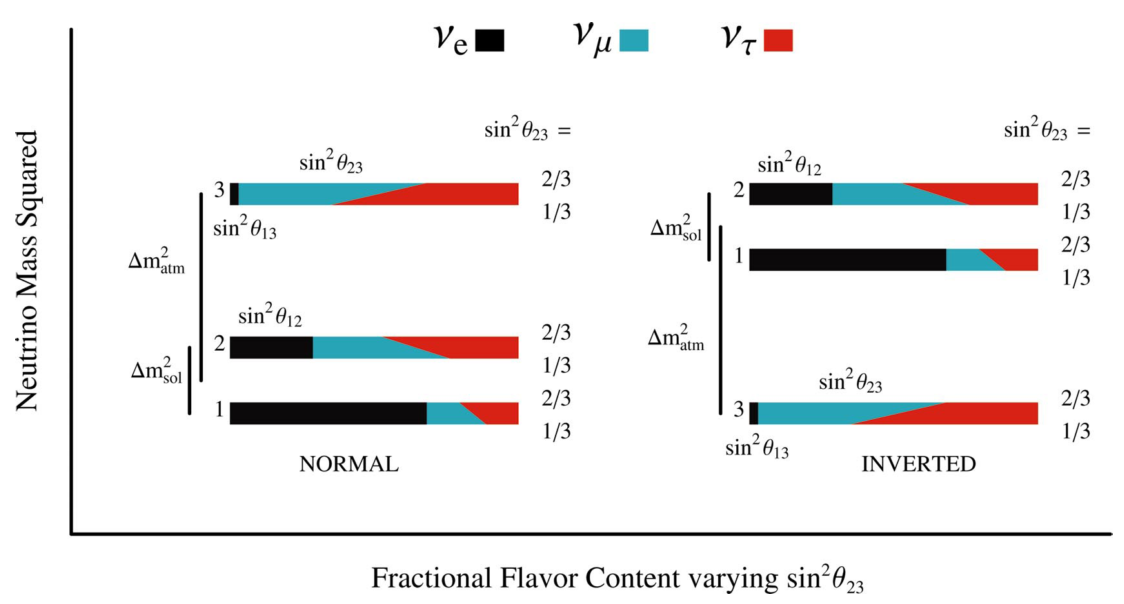
\includegraphics[width=\columnwidth]{assets/neutrino-mass-theta23.png}
\caption{Neutrino mass hierarchy. Mena, O., \& Parke, S. (2004). Unified graphical summary of neutrino mixing parameters. Physical Review D, 69(11), 117301.}
\label{fig:neutrino_mass_hierarchy}
\end{figure}


\begin{enumerate}
\item Mixing angles
\begin{align}
\sin^2 2\theta_{12} & = 0.857 \pm 0.024 \\
\sin^2 2\theta_{23} & > 0.95 \\
\sin^2 2\theta_{13} & = 0.095 \pm 0.010 \\
\end{align}
\item Masses (fig \ref{fig:neutrino_mass_hierarchy})
\begin{align}
\Delta m_{12}^2 &= \Delta m_{\mathrm{sol}}^2 = 7.53_{-0.18}^{+0.18} \times 10^{-5} \mathrm{eV}^2 \\
\lvert\Delta m_{31}^2\rvert & = \Delta m_{\mathrm{atm}}^2 = 2.44_{-0.06}^{+0.06}\times 10^{-3} \mathrm{eV^2} (\text{NH})
\end{align}
\item Typical oscillation frequencies
\begin{align}
   \omega_{v,21}=& \frac{\Delta m^2_{21}}{2E} = 1.90\times 10^{-4}  \mathrm{m}^{-1}  \frac{\delta m^2}{7.5\times 10^{-5}\mathrm{eV}^2} \frac{1\mathrm{MeV}}{E} \\
   \omega_{v,32} = & \frac{\Delta m^2_{32}}{2E} = 6.3\times 10^{-3} \mathrm{m}^{-1}  \frac{\Delta m^2_{32}}{2.5\times 10^{-3} \mathrm{eV}^2 } \frac{1\mathrm{MeV}}{E}.
\end{align}
\end{enumerate}







\subsection{Nuclear Reactions}


\begin{figure}[h]
\centering
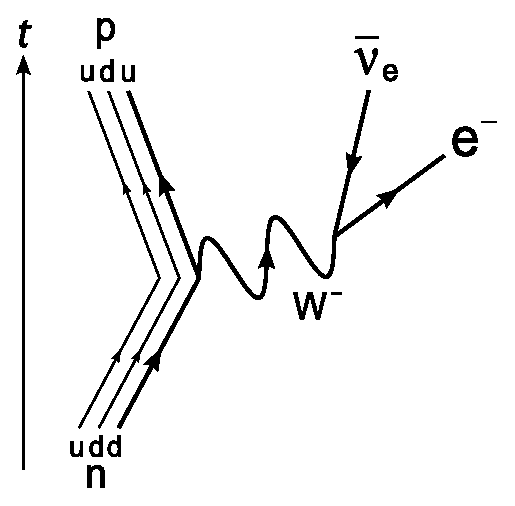
\includegraphics[width=\columnwidth]{assets/Beta_Negative_Decay.eps}
\caption{Feynman diagram of beta decay. The charged current weak interaction boson in this case is a $W^-$. Credit: Joel Holdsworth, within public domain.}
\label{fig:Beta_Negative_Decay}
\end{figure}





\begin{table}[ht]
\centering
\caption{Neutrino related nuclear or leptonic reactions}
 \begin{tabular}{|c | c | c|}
 \hline
 Reaction & Equation & Boson   \\ [0.5ex]
 \hline
 Electron emission & ${}^A_Z X \to {}^A_{Z+1}X + e^- +\bar \nu_e$ & $W$  \\
 Positron emission & ${}^A_Z X \to {}^A_{Z-1}X + e^+ + \nu_e$ & $W$  \\
 Electron capture & ${}^A_Z X + e^- \to {}^A_{Z-1}X  + \nu_e$ &  $W$ \\
 Positron capture & ${}^A_Z X + e^+ \to {}^A_{Z+1}X  + \bar\nu_e$ &  $W$ \\
 [0.5ex]
 \hline

 Electron annihilation &  $e^- + e^+  \to \nu_e + \bar\nu_e $  & $W$ \\
 Electron annihilation &  $e^- + e^+  \to \nu + \bar\nu $  & $Z$ \\
 [0.5ex]
 \hline

  Neutrino capture & ${}^A_{Z}X + \overset{(-)}{\nu_e} \to {}^A_{Z\mp 1}X + e^\pm $ & W\\
  [1ex]
 \hline
 $e^-\nu$ scattering & $e^- + \overset{(-)}{\nu_e} \to e^- + \overset{(-)}{\nu_e} $ &  $W$ \\
 $e^-\nu$ scattering & $e^{\pm} + \overset{(-)}{\nu_e} \to e^{\pm} + \overset{(-)}{\nu_e} $ &  $Z$ \\
 Neutrino scattering & $ {}^A_Z X + \overset{(-)}{\nu} \to {}^A_Z X + \overset{(-)}{\nu} $ &  Z\\
 [0.5ex]
 \hline

 Bremsstrahlung & $N+N\rightleftharpoons N+N + \nu + \bar\nu$ & \\
 Annihilation & $e^+e^- \rightleftharpoons \nu + \bar \nu$   & \\
 Neutrino annihilation & $\nu + \bar \nu  \rightleftharpoons \nu + \bar \nu $   &  \\
 [0.5ex]
 \hline
 \end{tabular}
\label{table:Neutrino_Reactions}
\end{table}



\subsection{Neutrino Mixing}

\begin{figure}
\centering
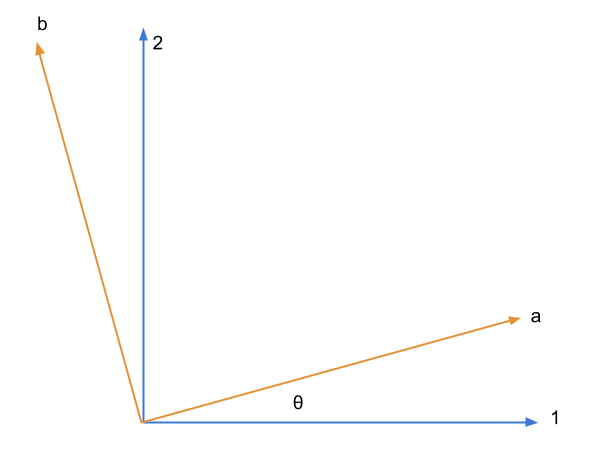
\includegraphics[width=\columnwidth]{assets/neutrinoMixingAngle.png}
\caption{Neutrino mixing. Blue states ($\{1,2\}$) are the VACUUM energy basis while the orange states ($\{a,b\}$) are the flavor basis. Blue: flavor basis; Red: propagation basis.}
\label{fig:neutrinoMixingAngle}
\end{figure}

The two basis are related to each other through a unitary matrix $\mathbf{U}$,

\begin{equation}
     \begin{pmatrix}
     \ket{\nu_e} \\
     \ket{\nu_x}
     \end{pmatrix} =
     \mathbf{U}
     \begin{pmatrix}
     \ket{\nu_1} \\
     \ket{\nu_2}
     \end{pmatrix},
\end{equation}


where

\begin{equation}
     \mathbf{U}=\begin{pmatrix}
     \cos \theta & \sin \theta \\
     -\sin \theta & \cos \theta
     \end{pmatrix}.
\end{equation}

One thing to notice is that the relation of the amplitude has the same transformation

\begin{equation}
     \begin{pmatrix}
     \psi_e \\
     \psi_x
     \end{pmatrix} =
     \mathbf{U}
     \begin{pmatrix}
     \psi_1 \\
     \psi_2
     \end{pmatrix},
\end{equation}

where the amplitude is define as the components of a state in a certain basis.

\begin{equation}
     \ket{\Psi} = \begin{pmatrix}
      \psi_e  & \psi_x
     \end{pmatrix} \begin{pmatrix}
     \ket{\nu_e} \\
     \ket{\nu_x}
     \end{pmatrix} =  \begin{pmatrix}
      \psi_1  & \psi_2
     \end{pmatrix} \begin{pmatrix}
     \ket{\nu_1} \\
     \ket{\nu_2}
     \end{pmatrix}.
\end{equation}



\subsection{Hamiltonian and Basis}


\subsubsection{Basis}

Rotation from a Hamiltonian diagonalized basis wave function $\Psi_v$ to flavor basis wave function $\Psi_f$ is

\begin{equation}
\Psi_f = R_{d2f}(\theta_x) \Psi_d,
\end{equation}

where $d$ can be $v$ for vacuum eigenbasis, $m$ for matter eigenbasis and

\begin{equation}
R_{d2f}(\theta_x) = \begin{pmatrix} \cos\theta_x & \sin \theta_x \\ -\sin \theta_x & \cos \theta_x \end{pmatrix}.
\end{equation}

Matter mixing angle $\theta_m$ is determined through

\begin{align}
\sin 2\theta_m &= \frac{\sin 2\theta_v}{ \sqrt{ \left(\frac{\lambda}{\omega_v}\right)^2 + 1 - 2 \frac{\lambda}{\omega_v}\cos 2\theta_v } } , \\
\cos 2\theta_m &= \frac{ \cos 2\theta_v - \lambda/\omega_v  }{ \sqrt{\left( \frac{\lambda}{\omega_v} \right) ^2  +1 - 2 \frac{\lambda}{\omega_v} \cos 2\theta_v } }, \\
\tan 2\theta_m &= \frac{\sin 2\theta_m}{\cos 2\theta_m - \lambda/\omega_v} ,
\end{align}

where $\lambda = \sqrt{2}G_F n_e$.


\subsubsection{Hamiltonian}

With the appearance of matter perturbation $\lambda (x) = \lambda_0 + \delta \lambda(x)$ to the system, we have the Hamiltonian in vacuum basis

\begin{equation}
    \mathbf{H_v} =  {\color{blue} -\frac{\omega_v}{2} \sigma_3 }  { \color{red} + \frac{\lambda (x)}{ 2 } \cos 2\theta_v \sigma_3 + \frac{\lambda(x)}{2} \sin 2\theta_v \sigma_1 } .
\end{equation}

In flavor basis,

\begin{equation}
    \mathbf{H_f} = {\color{blue}\frac{\omega}{2}( -\cos2\theta \sigma_3 + \sin 2\theta \sigma_1 )  } {\color{red} + \frac{\lambda(x)}{2} \mathbf {\sigma_3}}   .
\end{equation}


In background matter potential $\lambda_0$ basis

\begin{equation}
    \mathbf{H_{\bar m} } = -\frac{\omega_m}{2} \sigma_3 + \frac{\delta \lambda(x)}{2} \cos 2\theta_m \sigma_3 - \frac{\delta \lambda}{2} \sin 2\theta_m \sigma_1 ,
\end{equation}

where $\omega_m = \omega_v \sqrt{ \left( \frac{\lambda}{\omega_v} \right) ^2  +1 - 2 \frac{\lambda}{\omega_v} \cos 2\theta_v  }$.


The caveat is the position/time dependence of the matter potential leads to position/time dependent transformation of the wave function which will cause an term in the Hamiltonian of the form

\begin{equation}
     - i \mathbf{U}^\dagger (x) \frac{\partial}{\partial x} \mathbf{U}(x).
\end{equation}




\subsubsection{Physics of Neutrino Oscillation}


\begin{enumerate}
    \item Nature of neutrino oscillation
    \item MSW effect
    \item Collective oscillation
    \item Gravitation effect on neutrino oscillations
    \item Kinetic equation ($\nu\bar\nu$ pairing correlations?)
\end{enumerate}


\subsubsection{Applications of Neutrino Oscillation}


\begin{enumerate}
\item Supernova shock revive
\item Accretion disc
\item Cosmology
\item {\color{darkgray}Tomography}
\item {\color{gray}Detection of nuclear activities}
\end{enumerate}

\subsubsection{Big Questions}

\begin{enumerate}
    \item Are neutrinos Majorana or Dirac?
    \item What is the mass hierarchy?
\end{enumerate}


%%% Numerical

\section{Numerical}

\subsection{Writing Code}


\begin{enumerate}
\item Reduce quantities to dimensionless;
\item Always calculate the corresponding value of reduced quantities in suitable units.
\end{enumerate}

\subsection{Limits}

\begin{enumerate}
\item Simple cases where analytical is possible;
\item Verified numerical calculations had previously.
\end{enumerate}



\subsection{Zen of Python}

\verb+import this+


\subsection{Check You Code (Neutrino)}
Check the code step by step:

\begin{enumerate}
\item Vacuum oscillation amplitude and frequency
\item Constant matter potential oscillation amplitude and frequency
\item MSW resonance
\end{enumerate}








\end{multicols}

\end{document}
